\documentclass{6046}

\usepackage{tikz}
\usepackage{float}
\usepackage{enumitem}

\author{Matthew Feng}
\problem{9}
\collab{Alex Guo}

\begin{document}

\section*{Problem 1}
\subsection*{(a)}
First, we want to show
that SKIPPING-STONES is in NP. To do this,
we must demonstrate that given a
{\it certificate} or {\it solution}, we
can verify that the solution is correct in
polynomial time.

Given the moves to make, we can simply construct
the board and run through the moves, each move
taking at most $O(n)$ time. Finally, verifying
that the solution is correct (i.e. checking
that each row has a stone) can be done in
$O(n^2)$ time. Thus, verification may
be completed in polynomial time (given
a polynomial sized solution),
and thus SKIPPING-STONES is in NP.

\subsection*{(b)}
In order to prove SKIPPING-STONES is NP-hard, we
will prove the following
reduction:
$$\text{3-SAT} \le_P \text{SKIPPING-STONES}$$
In other words, we will transform an instance
of the 3-SAT problem into an instance of
SKIPPING-STONES using polynomial time, such
that if an efficient algorithm for SKIPPING-STONES
existed, then we would likewise have an
efficient algorithm for 3-SAT (which,
to our knowledge, does not exist).

Suppose our instance of 3-SAT has $K$ clauses
and $L$ literals.

If we have more clauses than literals, our
SKIPPING-STONES board will be of size
$K \times K$. Conversely, if we have more literals
than clauses, the board will have shape
$L \times L$.

We can imagine the board as follows:
\vspace{-1em}
\begin{itemize}[noitemsep]
    \item Each column corresponds a literal $x_j$.
    \item Each row corresponds to a clause $c_i$.
    \item If we have more literals than clauses,
    let the additional $L - K$ rows be a
    duplicate of clause $c_K$ (i.e. duplicate
    of row $K$); this is simply
    to follow the rules that the board must be square,
    and has no real meaning.
\end{itemize}

Using this construction, we can place stones
on the board according to the following rules:
\vspace{-1em}
\begin{itemize}[noitemsep]
    \item Let black stones represent {\bf False}
    truth values, and white stones represent
    {\bf True} truth values.
    \item For each clause $c_i = (a \vee b \vee c)$,
    place stones in corresponding to literals
    $a$, $b$, and $c$, placing a white stone
    where the literal is the same as the column
    label (e.g. $a$), or a black stone
    where the literal is a negation of the column
    label (e.g. $\bar{a}$).
    \item Otherwise, the space on the board should
    be left empty (i.e. literal $x_j$ doesn't appear
    in clause $c_i$).
\end{itemize}

We claim that this construction is an
instance of SKIPPING-STONES such that when
solved, yields a valid setting of the literals
that solves the 3-SAT problem.

We can see this because solutions to SKIPPING-STONES
only have a single color in each column, corresponding
to a single truth value for each literal. Solutions
must also have one stone per row; this is equivalent
to requiring that each clause having at least
one literal satisfying the clause.

Formally, we can turn any solution to the SKIPPING-STONES
problem into a valid solution for the 3-SAT,
by simplying assigning literal $x_j$ to {\bf True}
if the stones in column $x_j$ are all white, or $x_j$ to
{\bf False} if all the stones are black (if no stones
are in column $x_j$, then there does not exist a valid
solution). Likewise, given a valid assignment of the
literals, we know which stones to remove from
each column, such that we can solve the SKIPPING-STONES
problem.

Since it only took us $O(n^2), n = \max(K, L)$ time
to construct the SKIPPING-STONES board and place
the stones, the reduction can be performed in polynomial
time.

Thus, if an efficient algorithm exists for SKIPPING-STONES,
then we would be able to solve 3-SAT efficiently as well.
However, since we do not believe the latter to be the
case, we conclude that the former assumption is false;
that is, SKIPPING-STONES does not have an efficient,
polynomial time algorithm.

\section*{Problem 2}
\subsection*{(a)}
Again, we first want to demonstrate that
SCHEDULING is in NP as the first step
to proving that SCHEDULING is NP-complete.
Our approach again is to show that given
a {\it certificate}, we can verify its
validity in polynomial time.

Given a potentially valid schedule,
we can simply iterate over each student
$s$, looping through all the pairs of
classes that student $s$ is taking,
and verify that every pair does not conflict.
Since this can be done $O(|S||C|^2)$, where
$S$ is the set of all students and $C$ the
set of all classes, our verification
algorithm runs in polynomial time,
which shows that SCHEDULING is indeed in NP.

\subsection*{(b)}
In order to prove that SCHEDULING is NP-hard, we
first show that it is the equivalent problem
as graph 3-colorability (3-COLOR). In other words,
we want to transform an instance of SCHEDULING
into an instance of 3-COLOR, such that the
solution to 3-COLOR directly translates
into the solution for SCHEDULING.

Given the list of students $S$ and the classes
$C_s$ each student $s \in S$ is taking, and a list of classes
$C = \bigcup_{s \in S} C_s$, we can build an instance of the 3-COLOR problem
such that the solution to the 3-COLOR yields a solution
to SCHEDULING.

The goal is to build a graph $G$
whose coloring represents an exam scheduling.
In particular, represent each of the three
different exam blocks with a different color
(e.g. \{red, green, blue\}), such that
for any student, all the classes they are taking
are colored differently.

First, we can construct a node $\hat{c}_i$ for
each class $c_i \in C$.

Then, for every student $s_j \in S$ and their list of
classes $C_{s_j}$, build edge $(\hat{c}_a, \hat{c}_b)$, $\forall
c_a, c_b \in C_{s_j}, c_a \neq c_b$. These edges
encode the fact that no two classes can have exams
at the same time, otherwise student $s_j$ would be taking
two exams at the same time.

If the resulting graph $G$ has a valid 3-coloring, then
there does exist a feasible exam schedule. We can see
this in two steps:
\begin{itemize}
    \item Given the 3-coloring, simply assign each class
    to the exam block determined by its coloring. Since
    exam conflicts were defined by the edges, and
    graph coloring ensures that the endpoints of
    edges always have different colors, there cannot
    exist any exam conflicts.
    \item Given a valid exam scheduling, we can
    construct a valid 3-coloring on the graph $G$
    by assigning all nodes representing classes
    in the same exam block the same color. Again,
    because the edges represent exam conflicts,
    and the exam schedule is valid, the colors
    of the endpoints of every edge should be different,
    satisfying the requirement for a valid coloring. Since
    only three exam blocks exist, only three colors will
    be used, making it a valid 3-coloring.
\end{itemize}

Thus, we can see that SCHEDULING and 3-COLOR are equivalent
problems.

\subsection*{(c)}
Now that we know SCHEDULING and 3-COLOR are equivalent,
we want to show the following reduction can be peformed
in polynomial time:
\[
    \text{3-SAT} \le_P \text{3-COLOR}
\]
Given an instance of 3-SAT with $K$ clauses 
and $L$ literals, we need to build an instance of 3-COLOR,
such that the existence of a valid solution to
3-COLOR implies the existence valid setting
of the $L$ literals that satisfies all $K$ clauses
in 3-SAT.

First, we need some way of mapping colorings to truth values.
We can do this as follows: for every literal $x$,
construct a triangle of nodes $x_T$, $x_F$, $B$, where
$B$ is a common node shared among all triangles. We can
then imagine that three ``colors'' in our graph will be
\{T, F, B\}. Any node colored ``T'' takes on the truth
value {\bf True}, while any node colored ``F'' takes
on the truth value {\bf False}, and nodes colored ``B''
should not map to any literal.

Next, we show that given a clause $a \vee b \vee c$,
we can add edges to the node representation of literals
given by the previous paragraph to constrain
the coloring of a special node $x_{abc}$ that will
hold the truth value of $a \vee b \vee c$.

Consider the following construction:

\begin{figure}[H]
\begin{center}
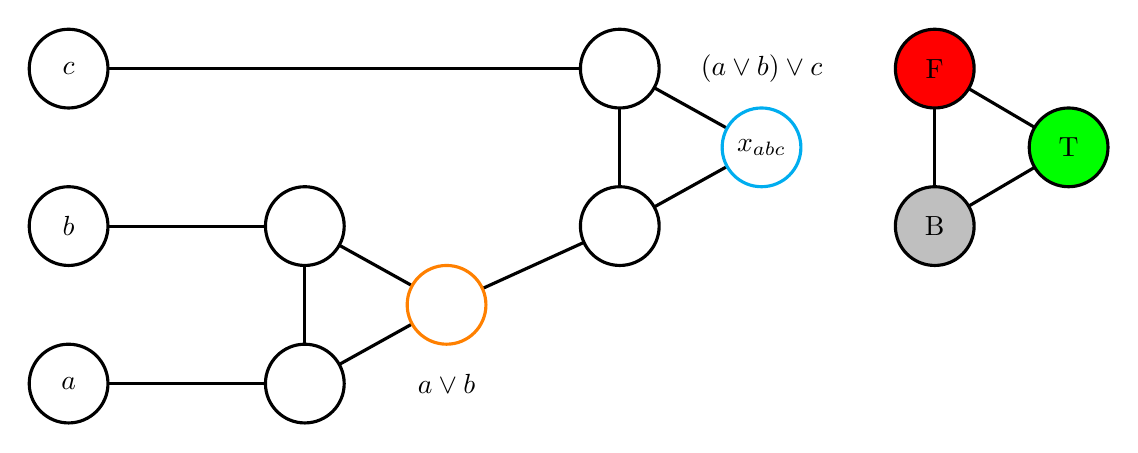
\begin{tikzpicture}
    % a, b input lines
    \draw [line width=0.4mm] (-10, 0) -- (-7, 0);
    \draw [line width=0.4mm] (-10, 2) -- (-7, 2);

    % triangle 1
    \draw [line width=0.4mm] (-7, 0) -- (-7, 2);
    \draw [line width=0.4mm] (-7, 0) -- (-5.2, 1);
    \draw [line width=0.4mm] (-7, 2) -- (-5.2, 1);

    % triangle 2
    \draw [line width=0.4mm] (-3, 2) -- (-3, 4);
    \draw [line width=0.4mm] (-3, 4) -- (-1.2, 3);
    \draw [line width=0.4mm] (-3, 2) -- (-1.2, 3);
    
    % c, (a v b) inputs to triangle 2
    \draw [line width=0.4mm] (-10, 4) -- (-3, 4);
    \draw [line width=0.4mm] (-5.2, 1) -- (-3, 2);

    % triangle 2 connection to F, B
    % \draw [line width=0.4mm] (-1.2, 3) -- (1, 2);
    % \draw [line width=0.4mm] (-1.2, 3) -- (1, 4);

    % T, F, B triangle
    \draw [line width=0.4mm] (2.7, 3) -- (1, 2);
    \draw [line width=0.4mm] (2.7, 3) -- (1, 4);
    \draw [line width=0.4mm] (1, 2) -- (1, 4);

    \draw [line width=0.4mm, fill=white] (-10, 0) circle [radius=0.5];
    \node[] at (-10, 0) {$a$};
    \draw [line width=0.4mm, fill=white] (-10, 2) circle [radius=0.5];
    \node[] at (-10, 2) {$b$};
    \draw [line width=0.4mm, fill=white] (-10, 4) circle [radius=0.5];
    \node[] at (-10, 4) {$c$};

    \draw [line width=0.4mm, fill=white] (-7, 0) circle [radius=0.5];
    \draw [line width=0.4mm, fill=white] (-7, 2) circle [radius=0.5];
    \draw [line width=0.4mm, fill=white, draw=orange] (-5.2, 1) circle [radius=0.5];
    \node[] at (-5.2, 0) {$a \vee b$};

    \draw [line width=0.4mm, fill=white] (-3, 4) circle [radius=0.5];
    \draw [line width=0.4mm, fill=white] (-3, 2) circle [radius=0.5];
    \draw [line width=0.4mm, fill=white, draw=cyan] (-1.2, 3) circle [radius=0.5];
    \node[] at (-1.2, 4) {$(a \vee b) \vee c$};
    \node[] at (-1.2, 3) {$x_{abc}$};

    \draw [line width=0.4mm, fill=lightgray] (1, 2) circle [radius=0.5];
    \node[] at (1, 2) {B};
    \draw [line width=0.4mm, fill=red] (1, 4) circle [radius=0.5];
    \node[] at (1, 4) {F};
    \draw [line width=0.4mm, fill=green] (2.7, 3) circle [radius=0.5];
    \node[] at (2.7, 3) {T};
\end{tikzpicture}
\end{center}
\end{figure}

The construction has the two following properties
that allow it to guarantee that $x_{abc}$ is
colored accordingly:
\begin{itemize}
    \item When $a$, $b$, $c$ are all colored ``F'' (noting
    that they are also connected to their respective
    triangles as previously described but not shown),
    the only color that $x_{abc}$ may have is ``F''.
    \item If any of $a$, $b$, or $c$ is colored ``T'',
    then there exists some coloring of the intermediate
    nodes such that $x_{abc}$ can be colored ``T''.
    We can force $x_{abc}$ to be colored as such by adding
    edges $(x_{abc}, F)$ and $(x_{abc}, B)$, which
    also has the side effect of invalidating
    all colorings if $a$, $b$, $c$ are all colored ``F'',
    since $x_{abc}$ will be forcibly connected
    to a node pre-colored ``F''.
\end{itemize}

Thus, this small subgraph allows us to map
the existence of a valid coloring to the existence
of a valid setting of $a$, $b$, $c$ such that
that clause is satisfied.

Now we build $k$ of these ``subgraphs'', one for
each clause, where all the nodes
highlighted in blue in the figure connect to
common nodes $F, B$, and that $B$ connects to
the literals in a triangular fashion described earlier
(i.e. $(B, x_T, x_F)$).

If a valid coloring exists in this final graph, then
every subgraph must have a valid coloring, which means
all $k$ clauses must be satisfied.

This reduction is correct because, by taking
the nodes colored ``T'' in the $(B, x_T, x_F)$
triangles, we get a assignment
of variables that solves our 3-SAT problem, since
we had previously demonstrated the one-to-one mapping
between clause and coloring. Conversely,
given a valid assignment of variables,
we can construct a valid coloring of the graph
by assigning all the nodes corresponding to
true literals with the color ``T''.

The reduction can be constructed in polynomial time since
we do constant amount of work constructing nodes
and edges for each of the $k$ clauses.

Thus, if we had an efficient algorithm to 3-COLOR, we
could efficiently solve 3-SAT. However, to our knowledge,
no such algorithm exists for 3-SAT, and thus
no such algorithm exists for 3-COLOR.
\end{document}

